\section{BigchainDB Implementation Details}\label{sec:implementation}

\subsection{Choice of Distributed DB}
The BigchainDB design is flexible enough to have been built on top of a wide variety of existing distributed DBs.
Of course, we had to choose a first one to build on.
To select which, we first did benchmarking, then added additional criteria.

There are $>100$ DBs to choose from, listed for example at \cite{nosql} and \cite{toad2015toad}.
This was our shortlist: Cassandra \cite{cassandra}, HBase \cite{hbase}, Redis \cite{redis}, Riak \cite{riak}, MongoDB \cite{mongodb}, RethinkDB \cite{rethinkdb}, and ElasticSearch \cite{elasticsearch}.
Each of these DBs uses Paxos or a Paxos descendant such as Raft \cite{ongaro2014raft}.

First, we did preliminary performance investigation of the DBs in our shortlist: Each had $15-105$ writes/s per thread, $290-1000$ serial reads/s per thread, and $80-400$ reads/s per thread.

While there was some variation in performance among the DBs, the key thing to notice is that performance is per thread: performance improves as the number of threads increases.
This is different than traditional blockchain technologies, where performance stays flat or worsens.

Given that all DBs tested had good scalability properties, we realized that other criteria were even more important. In particular:
\begin{enumerate}
 \item \textbf{Consistency.} Distributed DBs must make a trade-off between performance and consistency (in the CAP theorem \cite{wiki_cap} sense, not ACID sense \cite{wiki_acid}). For a blockchain, consistency means trustworthy ordering of transactions, so we prefer DBs with strong consistency guarantees.
 \item{\textbf{Automatic Change Notifications.} One way for a node to find out if a change has happened in a DB is to ask it on a regular basis (i.e. polling), but that’s not as efficient as having the DB automatically notify the node of changes.
  We wanted a DB with automatic change notifications as a standard feature.
  
  \medskip
  Automatic change notifications bring another benefit: they improve tamper-resistance (beyond what a chain of hashes offers).
  If a hacker somehow manages to delete or update a record in the data store, the hashes change (like any blockchain).
  In addition, a datastore with automatic change notifications would notify all the nodes, which can then immediately revert the change and restore the hash integrity.}
\end{enumerate}

Of the options considered, we found that RethinkDB met our needs best.
It has strong consistency guarantees \cite{rethinkdb_consistency} and it offers automatic change notifications (“changefeeds”) as a standard feature \cite{rethinkdb_changefeeds}.
Therefore, we built the first version of BigchainDB on top of RethinkDB.

RethinkDB is a JSON (NoSQL) database with a flexible query language \cite{rethinkdb_faq}.
It is optimized for scalable realtime feeds, which is useful for collaborative apps, streaming analytics, multiplayer games, realtime marketplaces, and connected devices / IoT\footnote{IoT = Internet of Things}.
It is built in C++, is open source, and has a vibrant development community \cite{rethinkdb_github}.
If one wants full ACID support or strong schema enforcement, then a SQL database is a better choice; if one prefers availability over consistency then Riak \cite{riak} is a better choice \cite{rethinkdb_faq}.

In the future, we envision a variety of distributed databases being “blockchain-ified” according to the approach of this paper.
Every relational database, document store and graph store on the planet might someday have a blockchain version.

\subsection{BigchainDB Datastore Architecture}
Figure \ref{fig:bigchaindb_datastore_architecture} shows the architecture of the BigchainDB datastore, with three nodes as example. 
We run each node as an AWS\footnote{AWS = Amazon Web Services} t2.medium node (or otherwise). 
We use the RethinkDB storage backend, with a sharded cluster, and master/master-replication.

\noindent There are three key interactions with a node:
\begin{itemize}
 \item $\mathtt{big\_API}$ controls access to the datastore. It is through the $\mathtt{big\_API}$ where there is access for admin, applications, and any other clients. 
 \item $\mathtt{big\_trigger}$ verifies changes in the backlog, i.e. the UPDATE / DELETE calls. 
 \item $\mathtt{big\_processor}$ creates blocks of verified data from the backlog, and writes blocks to the bigchain.
\end{itemize}

\begin{figure}[!ht]
  \centering
  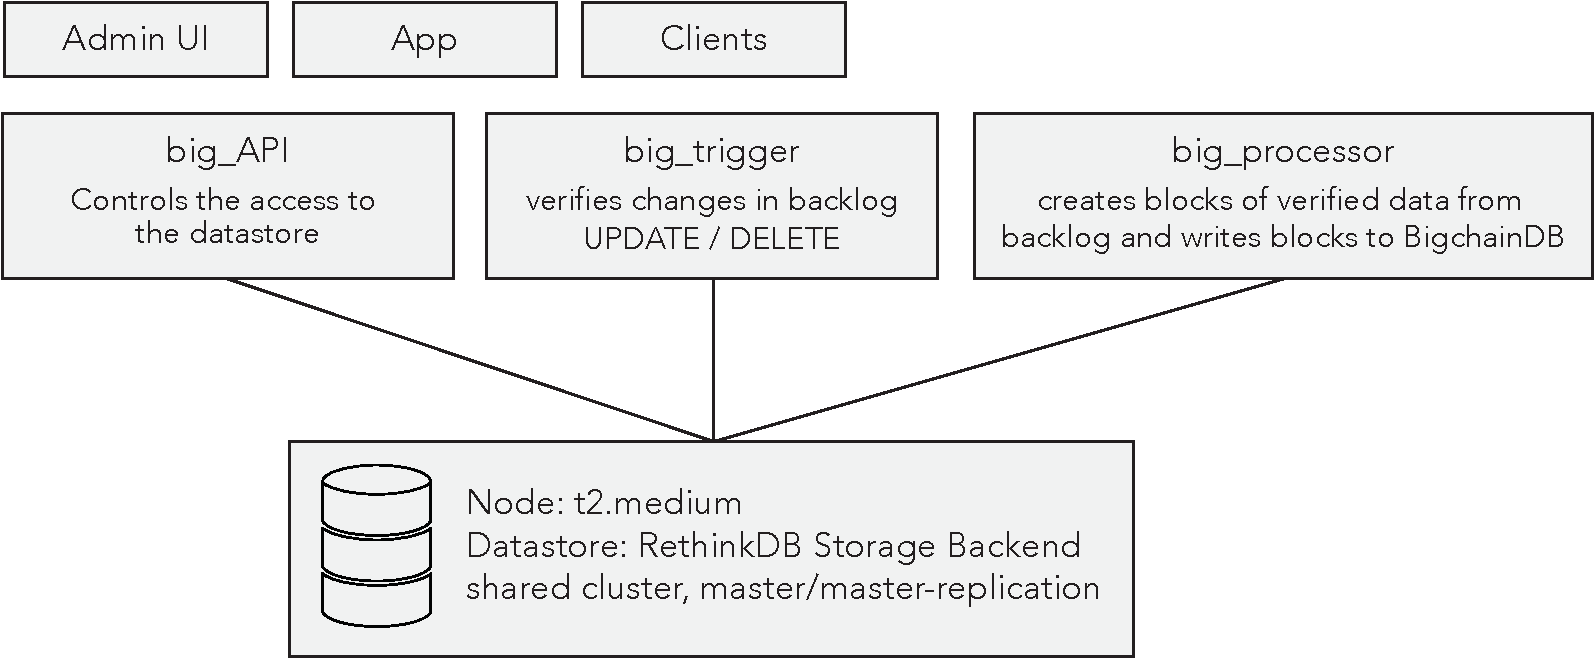
\includegraphics[width=\textwidth]{figure_9.pdf}
  \caption{BigchainDB datastore architecture.}
  \label{fig:bigchaindb_datastore_architecture}
\end{figure}

\subsection{BigchainDB Capacity}
Each t2.medium provides $48$ TB of storage, so the total capacity of $N$ nodes is $N$ times $48$ TB; with $32$ nodes, the total capacity is $1536$ TB, i.e. more than a Petabyte.
For quick reference, Figure \ref{fig:bigchain_capacity_vs_nodes} shows how total capacity depends on the number of nodes. 

\begin{figure}[!ht]
  \centering
  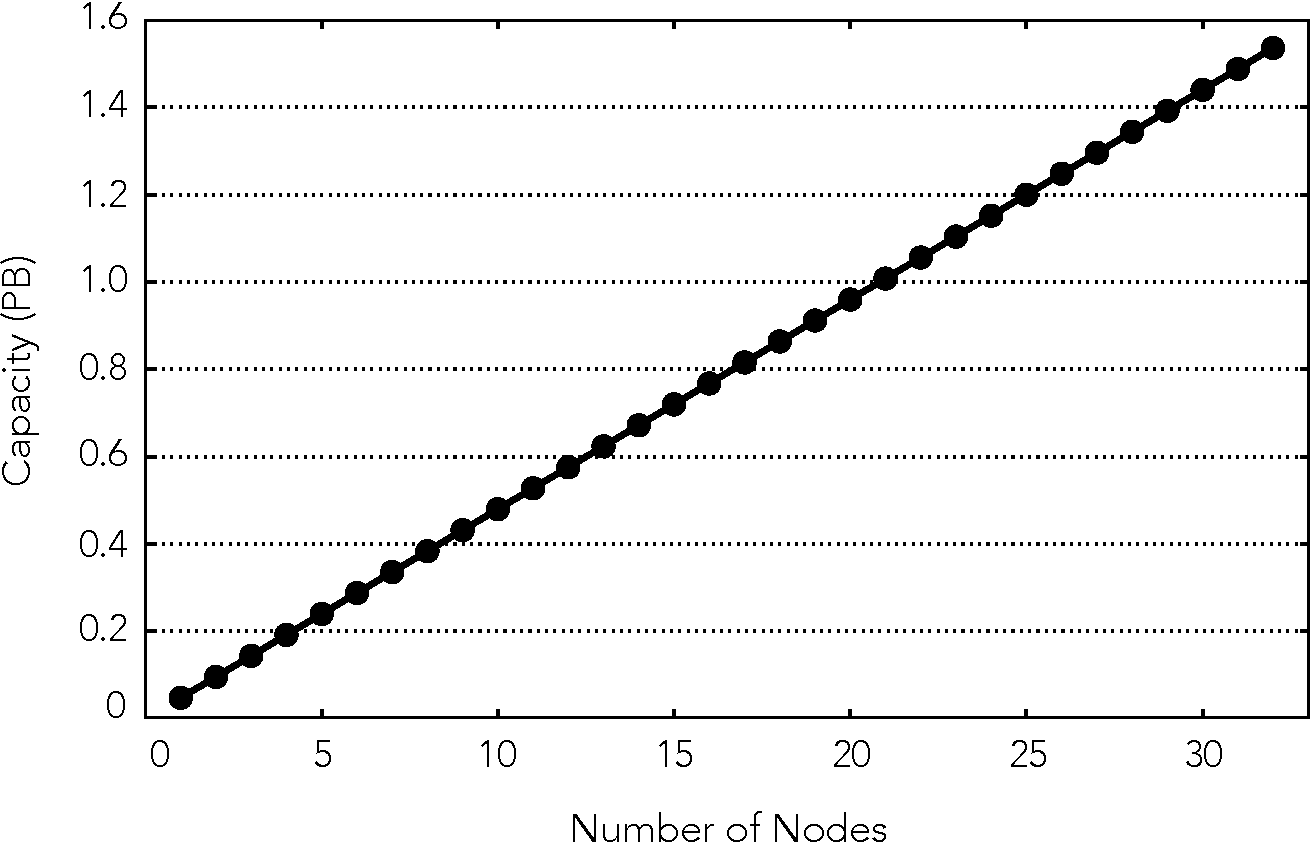
\includegraphics[width=0.8\textwidth]{figure_10.pdf}
  \caption{BigchainDB Capacity versus Number of Nodes. Each node adds another $48$ TB to the total storage capacity.}
  \label{fig:bigchain_capacity_vs_nodes}
\end{figure}

\subsection{Cryptography}

This section describes choices of cryptographic algorithms. 

\subsubsection{Hashes}

We hash using the SHA3-256 algorithm. We store the hex encoded hash in the BigchainDB. Here is a python implementation example, using pysha3\footnote{\url{https://bitbucket.org/tiran/pykeccak}}.

\begin{minipage}{\linewidth}
  \begin{lstlisting}[style=python]
  import hashlib 
  # monkey patch hashlib with sha3 functions 
  import sha3 
  data = "message" 
  tx_hash = hashlib.sha3_256(data).hexdigest()\end{lstlisting}
\end{minipage}

\subsubsection{Keys}
For signing and verifying signatures we are using the Elliptic Curve Digital Signature Algorithm (ECDSA) with $256$bit keys and the secp256k1 curve parameters, the same as used by Bitcoin and Ethereum.

The public-key or verification key are converted to string and hex encoded before storing them to BigchainDB.

\medskip
\noindent Here is a python implementation example, using \mbox{python-ecdsa}\footnote{\url{https://github.com/warner/python-ecdsa}}:

\begin{minipage}{\linewidth}
  \begin{lstlisting}[style=python]
  import binascii
  from ecdsa import SigningKey 
  # generate signing key in hex encoded form 
  sk = SigningKey.generate() 
  sk_hex = binascii.hexlify(sk.to_string()) 
  # get signing key from hex 
  sk = SigningKey.from_string(binascii.unhexlify(sk_hex))\end{lstlisting}
\end{minipage}


\subsection{Serialization}
We need to clearly define how to serialize a JSON object (RFC7159) to calculate the hash. 
The serialization should produce the same byte output independently of the architecture running the software.
If there are differences in the serialization hash validations will fail although the transaction is correct.

\medskip
\noindent Here is an example:

\begin{minipage}{\linewidth}
  \begin{lstlisting}[style=python]
  >>> a = r.expr({'a': 1}).to_json().run(b.connection)
  u'{"a":1}'
  >>> b = json.dumps({'a': 1}) 
  '{"a": 1}' 
  >>> a == b 
  False\end{lstlisting}
\end{minipage}

\medskip
\noindent We should provide the serialization and deserialization so that the following is always true.
\medskip
\noindent For example: 

\begin{minipage}{\linewidth}
  \begin{lstlisting}[style=python]
  >>> deserialize(serialize(data)) == data 
  True\end{lstlisting}
\end{minipage}


\subsubsection{Standard serialization for BigchainDB}
We are currently using the python JSON module, because it complies with the RFC.
We can specify the encoding, separators used and enforce it to order by the keys to make sure that we obtain maximum interoperability. 

\begin{minipage}{\linewidth}
  \begin{lstlisting}[style=python]
  import json 
  json.dumps(data, skipkeys=False, ensure_ascii=False, encoding="utf-8", separators=(',', ':'), sort_keys=True)\end{lstlisting}
\end{minipage}

\noindent The parameters mean: 
\begin{itemize}
 \item $\mathtt{skipkeys}$: With skipkeys $\mathtt{False}$ if the provided keys are not a string the serialization will fail. This way we enforce all keys to be strings
 \item $\mathtt{ensure\_ascii}$: The RFC recommends utf-8 for maximum interoperability. By setting $\mathtt{ensure\_ascii}$ to $\mathtt{False}$ we allow unicode characters and force the encoding to $\mathtt{utf-8}$. 
 \item $\mathtt{separators}$: We need to define a standard separator to use in the serialization. We did not do this different implementations could use different separators for serialization resulting in a still valid transaction but with a different hash e. g. an extra whitespace introduced in the serialization would still create a valid json object but the hash would be different
\end{itemize}

\subsubsection{Example}
Every time we need to perform some operation on the data like calculating the hash or signing/verifying the transaction, we need to use the previous criteria to serialize the data and then use the byte representation of the serialized data (if we treat the data as bytes we eliminate possible encoding errors e.g. unicode characters):

\begin{minipage}{\linewidth}
  \begin{lstlisting}[style=python]
  # calculate the hash of a transaction 
  # the transaction is a dictionary 
  tx_serialized = bytes(serialize(tx)) 
  tx_hash = hashlib.sha3_256(tx_serialized).hexdigest() 
  # signing a transaction 
  tx_serialized = bytes(serialize(tx)) 
  signature = sk.sign(tx_serialized) 
  # verify signature 
  tx_serialized = bytes(serialize(tx)) 
  vk.verify(signature, tx_serialized)\end{lstlisting}
\end{minipage}
